\documentclass[titlepage]{jsarticle}
\usepackage[dvips]{graphicx}
\usepackage{listings}
\usepackage{cprotect}
\usepackage{h31ec-exp}
\lstset{
  basicstyle={\ttfamily},
  identifierstyle={\small},
  commentstyle={\smallitshape},
  keywordstyle={\small\bfseries},
  ndkeywordstyle={\small},
  stringstyle={\small\ttfamily},
  frame={tb},
  breaklines=true,
  columns=[l]{fullflexible},
  numbers=left,
  xrightmargin=0zw,
  xleftmargin=3zw,
  numberstyle={\scriptsize},
  stepnumber=1,
  numbersep=1zw,
  lineskip=-0.5ex
}
\renewcommand{\lstlistingname}{ソースコード}
\makeatletter
\newcommand{\figcaption}[1]{\def\@captype{figure}\caption{#1}}
\newcommand{\tblcaption}[1]{\def\@captype{table}\caption{#1}}
\makeatother
\title{信号処理プログラミング}
\grade{4年32番}
\author{平田 蓮}
\team{}
\date{2020年6月18日}
\expdate{2020年5月21日, 5月28日, 6月4日, 6月11}
\coauthor{
}

\begin{document}
\maketitle
\section{目的}
    アナログ信号をディジタルデータに変換し, ディジタル機器で処理するために必要な起訴事項について学習し,
    C言語で基本的な信号処理プログラムを作成する.
    また音声フォーマットの一つであるWAVEファイルの構造を理解し, 音声データの入出力プログラムを作成する.

\section{周期関数の生成と可視化}
    正弦波のように一定周期ごとに同じ波形が繰り返される関数を\textbf{周期関数}と呼ぶ.
    よく知られている周期関数として, のこぎり波などがある.
    本節では周期関数に関する演習を行う.

    \paragraph{演習1-1} 任意の孤度$r$を区間$[0:2\pi]$に変換する関数\verb|rad|を作成せよ.

        作成した関数をソースコード\ref{src:rad}に示す.

        \begin{lstlisting}[caption=rad.c, label=src:rad]
double rad(double r) {
    if (r >= 0) {
        return fmod(r, 2 * PI);
    } else {
        return 2 * PI - fmod(-r, 2 * PI);
    }
}
        \end{lstlisting}

        $r$が正のときは$2\pi$との剰余を取る.
        $r$が負のときは, $r$を正数に変換し, $2\pi$と剰余をとったものを$2\pi$から引くことで変換している.

        図\ref{fig:rad}に横軸に$r$, 縦軸に\verb|rad(r)|を取ったグラフを示す.
        この図から, 変換がうまく行われていることがわかる.

        \begin{figure}[ht]
            \centering
            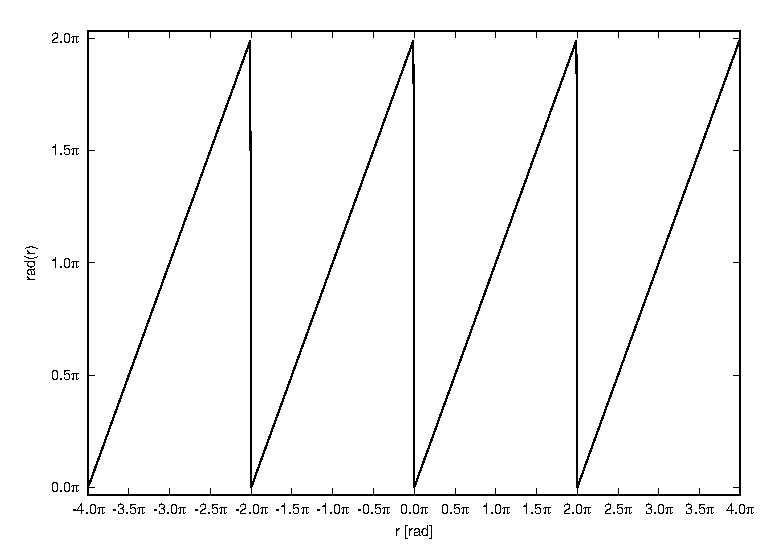
\includegraphics[width=12cm]{images/rad.eps}
            \cprotect\caption{\verb|rad|による変換}
            \label{fig:rad}
        \end{figure}

    \paragraph{演習1-2} 任意の孤度$r$に対して, のこぎり波の振幅値を求める関数\verb|saw|を作成せよ.

        作成した関数をソースコード\ref{src:saw}に示す.

        \begin{lstlisting}[caption=saw.c, label=src:saw]
double saw(double r) {
    return 1 - rad(r) / PI;
}
        \end{lstlisting}

        まず与えられた孤度$r$を演習1-1で実装した\verb|rad|を使い$[0:2\pi]$の範囲に変換する.

        $r$が$2\pi$の倍数の場合に1を取り, そこから傾き$-\frac{1}{\pi}$の形を繰り返すので,
        上記のように実装することができた.

        図\ref{fig:saw}にグラフを示す. うまくのこぎり波が現れていることがみてとれる.

        \begin{figure}[ht]
            \centering
            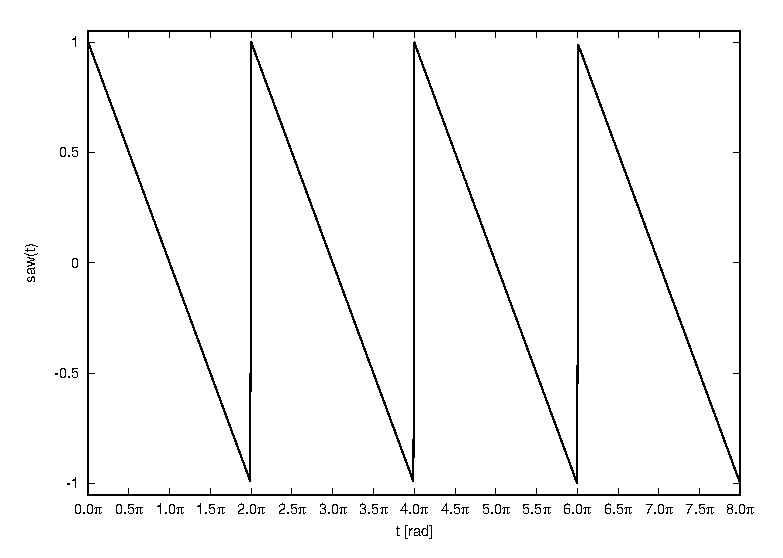
\includegraphics[width=12cm]{images/saw.eps}
            \cprotect\caption{\verb|saw|による変換}
            \label{fig:saw}
        \end{figure}

\section{サンプリング}
    アナログ信号波形をディジタルデータに変換する手法に\textbf{サンプリング}がある.
    本節では演習問題を通して実際にサンプリングの様子を観察する.

    \paragraph{演習2-1} リスト2のコードを解析し, 完成させよ. 振幅100, 周波数4Hzのデータを
    出力リダイレクションを使ってsin100f4.csvに出力せよ. このsin100f4.csvをgnuplotでグラフ化し,
    サンプリングの効果を確認せよ.

        まず, 完成させたリスト2のコード, sin10af1.cを出力部分を抜粋して掲載する.

        \begin{lstlisting}[caption=sin10af1.c, label=src:sin10af1]
for (t = 0; t <= TEND; t += DT) {
    r = 2 * PI * frq * t / 1000.0;
    vin = amp * sin(r) + BIAS;
    if (vin > 255) {
        vout = 255;
    } else if (vin < 0) {
        vout = 0;
    } else {
        vout = vin;
    }
    printf("%4f, %4d\n", t / 1000.0, vout);
}
        \end{lstlisting}

        4行目から10行目に渡って, クリッピングという処理を施してある.
        クリッピングをすることで, 出力用の変数(今回は8bitのchar型)に収まらない値を切り捨て,
        波形を維持することができる.

        図\ref{fig:sin100f4}にサンプリングしたデータを示す.
        実際に正弦波をサンプリングできていることがわかる.

        \begin{figure}[ht]
            \centering
            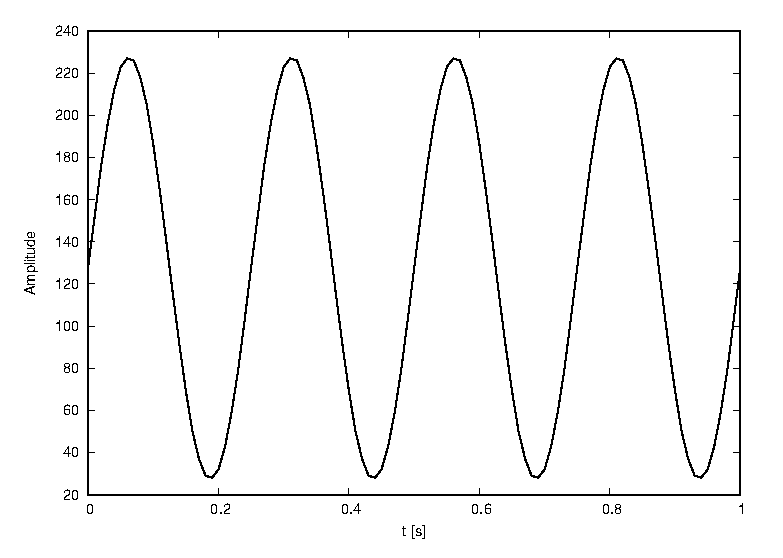
\includegraphics[width=12cm]{images/sin100f4.eps}
            \caption{振幅100, 周波数4Hzの正弦波}
            \label{fig:sin100f4}
        \end{figure}

    \paragraph{演習2-2} 振幅150, 周波数4Hzのデータsin150f4.csvを生成しその波形を確認せよ.
    波形に不具合があればその原因を考えて不具合を軽減するような修正を行え.
        
        今回は振幅が150なので, char型に収まらない数値をサンプリングすることになる.
        そこで, 演習2-1で実装したクリッピングが働く.

        図\ref{fig:sin150f4_1}, \ref{fig:sin150f_2}にクリッピングを施した前と後の波形を示す.
        この図からクリッピングの効果がみて取れる.
        クリッピングをしていない波形では, オーバーフローした値が波形の逆側に飛んでしまい,
        波形が崩れているが, クリッピングを施した方ではオーバーフローした値が切り捨てられ, 波形が維持できている.
        
        \begin{figure}[ht]
            \begin{minipage}{0.45\hsize}
                \centering
                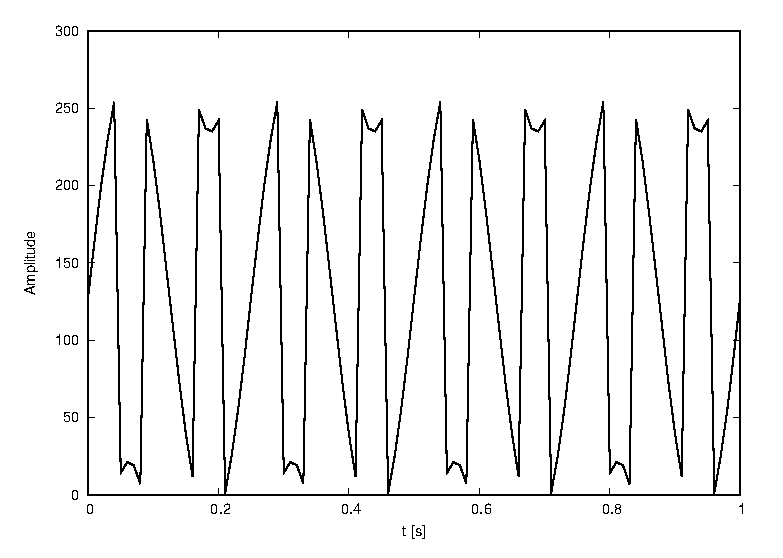
\includegraphics[width=9cm]{images/sin150f4_1.eps}
                \caption{振幅150, 周波数4Hzの正弦波(クリッピングなし)}
                \label{fig:sin150f4_1}
            \end{minipage}
            \begin{minipage}{0.45\hsize}
                \centering
                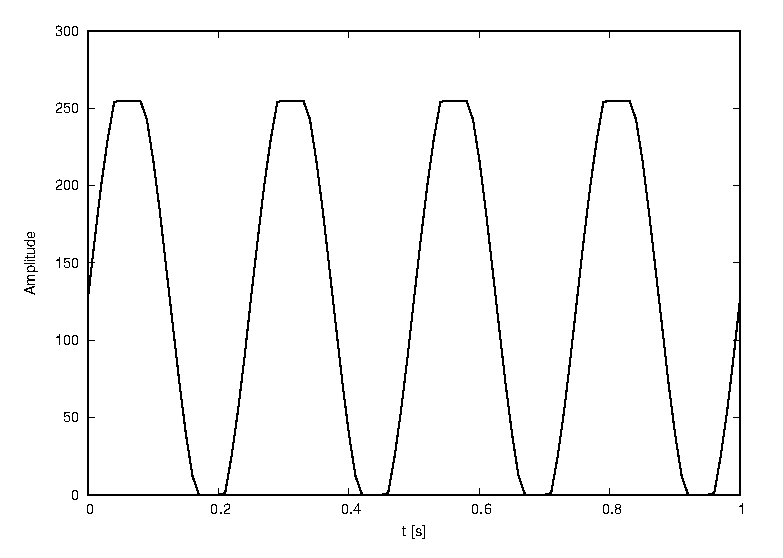
\includegraphics[width=9cm]{images/sin150f4_2.eps}
                \caption{振幅150, 周波数4Hzの正弦波(クリッピングあり)}
                \label{fig:sin150f4_2}
            \end{minipage}
        \end{figure}

\begin{thebibliography}{99}
    \bibitem{Electro} Electro-ワンチップマイコン http://laboratory.sub.jp/ele/13.html/
\end{thebibliography}

\end{document}
